\section{Симметрии и топология относительного движения}

В этом разделе исследуются симметрии системы и орбит, структура Жордана для тривиального мультипликатора \(\mu=1\) и топология относительного движения тел (числа обхода). Эти аспекты важны для понимания того, что является физическим механизмом переходов в семействе, а что — геометрическим следствием изменения амплитуды.

\subsection{Симметрии системы и орбит}
Уравнения движения в плоской задаче трёх тел с равными массами обладают группой симметрий, порождённой перестановками тел \(\sigma_{12}, \sigma_{13}, \sigma_{23}\) и поворотом на \(\pi\) (обозначим \(R_\pi\)). Все восемь элементов группы (включая композиции \(\sigma_{ij} \cdot R_\pi\)) проверены численно: для каждой из них выполняется тождество
\begin{equation}
    S \cdot f(X) = f(S \cdot X)
\end{equation}
с точностью до машинного нуля.

Для самих периодических орбит единственной нетривиальной симметрией оказалась
\begin{equation}
    X(T/2) = (\sigma_{13} \cdot R_\pi) \cdot X(0),
\end{equation}
то есть через половину периода орбита переходит в себя при перестановке тел 1 и 3, совмещённой с поворотом на \(\pi\). Тождество выполняется с точностью \(10^{-11}\) для орбит малой амплитуды и \(10^{-3}\) для орбит с большими амплитудами (что соответствует накопленной ошибке интегрирования на длинных периодах). Остальные элементы группы дают расстояние \(\sim |X_0|\), то есть не являются симметриями орбит.

\subsection{Структура Жордана для \(\mu=1\)}
Для тривиального мультипликатора \(\mu=1\) во всём семействе (кроме начальной точки \(gidx=0\), лежащей на самом равновесии) структура Жордана имеет вид
\begin{equation}
    J_2 + J_2,
\end{equation}
то есть матрица монодромии имеет две жордановы клетки размера 2. Это \textbf{стандартная} структура для однопараметрического семейства периодических орбит в гамильтоновой системе: две жордановы клетки отвечают сдвигу вдоль орбиты и сдвигу вдоль семейства. Скрытой симметрии, порождающей дополнительную кратность (как \(J_3\) или \(J_4\)), в семействе нет.

\subsection{Числа обхода: тела вокруг своих равновесий}
Были вычислены числа обхода траекторий каждого тела вокруг своей точки равновесия (тела 1 и 3 — вокруг \((\pm 1, 0)\), тело 2 — вокруг \((0,0)\)), а также числа обхода величин \(\rho_1\) и \(\rho_2\) вокруг точек столкновений. Результат:
\begin{itemize}
    \item число обхода каждого тела вокруг своего равновесия \textbf{всегда равно} \(w = -1\) для всех орбит семейства;
    \item число обхода \(\rho_2\) вокруг точки столкновения 1–2 всегда равно \(0\);
    \item число обхода \(\rho_1\) вокруг точки столкновения равно \(0\) в блоке \textit{unified} до \(gidx \approx 16111\), затем равно \(-1\); в блоке \textit{arclength} оно равно \(-1\) или \(-2\) с 45 переходами.
\end{itemize}
Полная симметрия тел 1, 2, 3 вокруг своих равновесий (\(w=-1\) у всех) подтверждает симметрию равных масс и является геометрическим свойством орбит Ляпунова.

\subsection{Интерпретация переходов числа обхода \(\rho_1\): \(0 \to -1\)}
Изменение числа обхода \(\rho_1\) вокруг точки столкновения с \(0\) на \(-1\) при \(gidx \approx 16111\) не является топологической бифуркацией в смысле смены класса орбиты. Это \textbf{геометрическое следствие роста амплитуды}: при увеличении амплитуды траектория \(\rho_1(t)\) начинает охватывать точку столкновения, и число обхода меняется скачком.

Порог по относительной глубине ямки для этого события составляет \(0.4110\), в то время как порог для переходов C \(\leftrightarrow\) R составляет \(0.4076\). Оба порога близки и соответствуют геометрическому условию «орбита начинает охватывать точку», а не какому-либо динамическому механизму.

\subsection{Связь числа обхода с устойчивостью}
Прямой связи между числами обхода и переходами C \(\leftrightarrow\) R не обнаружено: медианное расстояние между событиями составляет \(\sim 2300\) индексов, ни одного точного совпадения нет. Аналогично, корреляция \(\lambda\) с числом обхода после удаления влияния \(T\) оказывается слабой. В плоскости \((\text{depth}, \lambda)\) точки с \(w=-1\) и \(w=-2\) ложатся на одну и ту же кривую, то есть число обхода не является независимым параметром, а определяется амплитудой (глубиной ямы).

\begin{figure}[H]
    \centering
    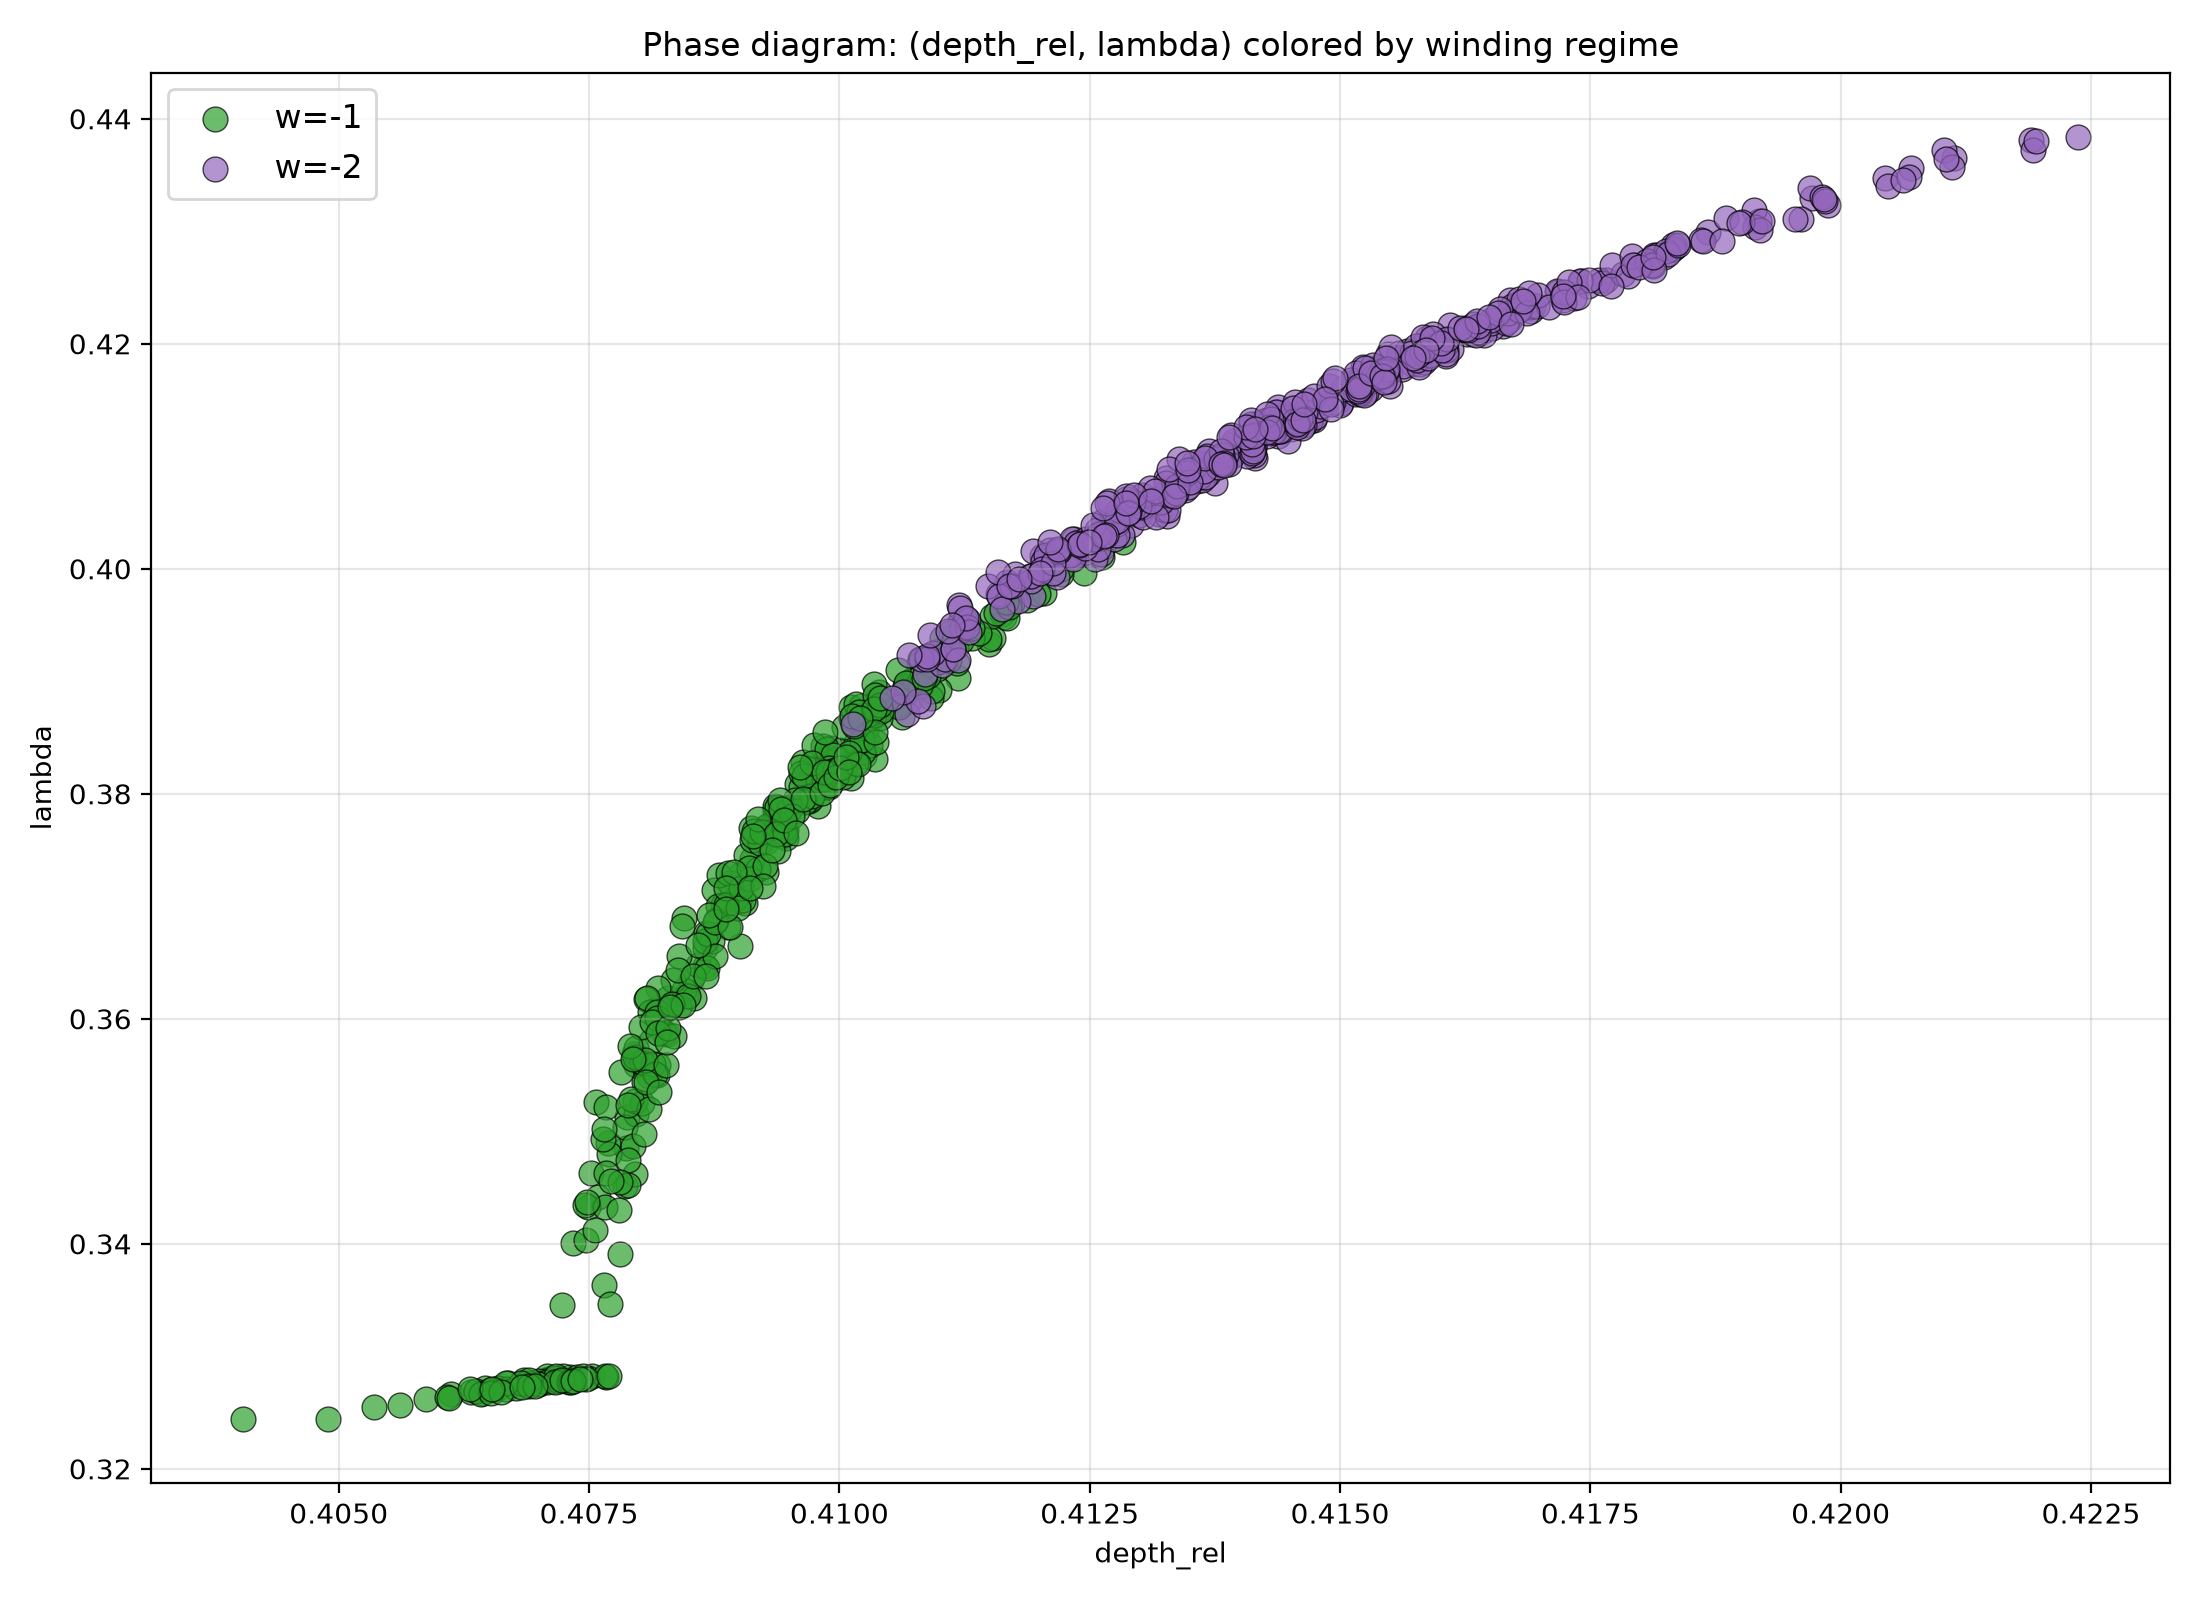
\includegraphics[width=0.8\textwidth]{67_phase_diagram.png}
    \caption{Фазовая диаграмма в плоскости \((\text{depth}, \lambda)\). Точки с разными числами обхода лежат на одной кривой, что указывает на отсутствие независимой связи между числом обхода и устойчивостью.}
    \label{fig:phase_diagram_winding}
\end{figure}

\begin{figure}[H]
    \centering
    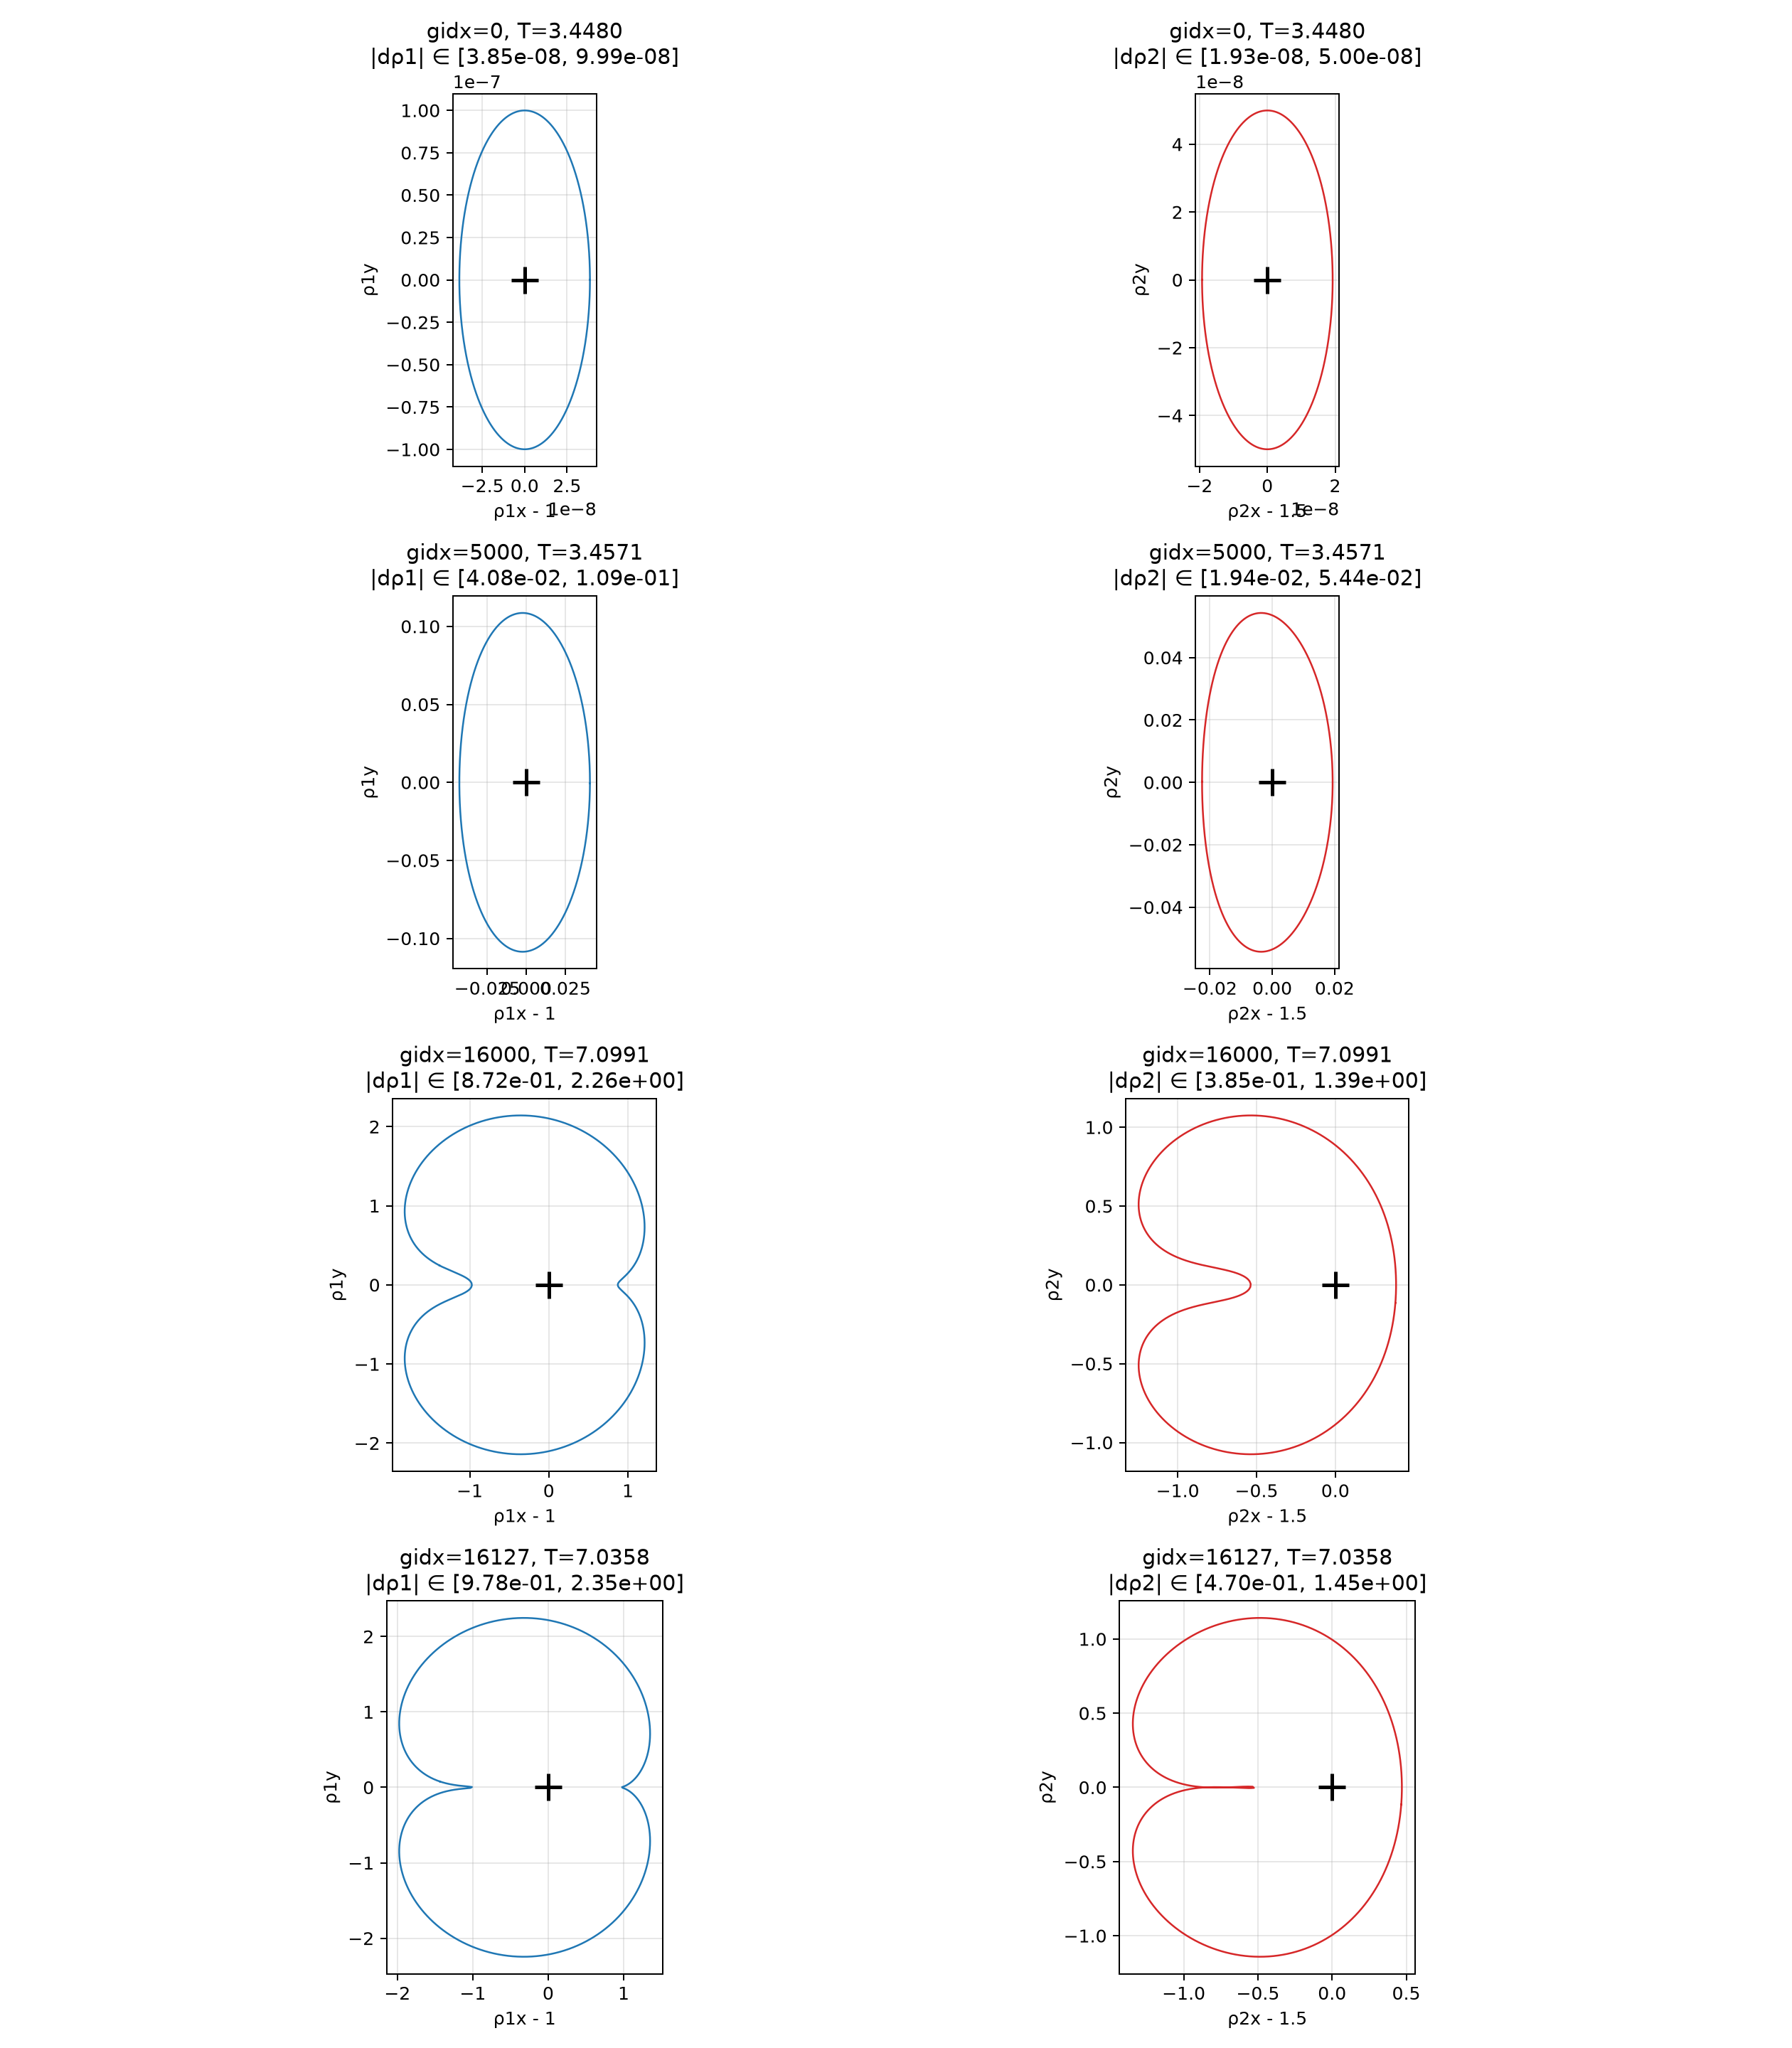
\includegraphics[width=0.85\textwidth]{88_libration_anatomy.png}
    \caption{Анатомия либрации: эллипс вокруг равновесия и восьмёрка. Число обхода каждого тела вокруг своего равновесия \(w=-1\) — следствие полного обхода за период.}
    \label{fig:libration_anatomy}
\end{figure}
